\documentclass[multi,crop=false,class=article]{standalone}
\onlyifstandalone{\usepackage{hyperref}
\usepackage{cleveref}
\usepackage[disable]{todonotes}
\presetkeys{todonotes}{inline, noline}{}
\usepackage{caption}
\usepackage{subcaption}
\usepackage{amsfonts}
\usepackage{theorem}
\usepackage{algorithm}
\usepackage{algpseudocode}
\theoremstyle{plain}
\theorembodyfont{\slshape}
\newtheorem{definition}{Definition}[section]
\usepackage{algorithm}
\usepackage{algpseudocode}
\usepackage{amsmath}
\usepackage{mathtools}
\usepackage{tikz}

\usetikzlibrary{automata,arrows}

%\DeclareCaptionType{algorithm}
\algdef{SE}[DOWHILE]{Do}{doWhile}{\algorithmicdo}[1]{\algorithmicwhile\ #1}%

% Math macros
\newcommand{\concat}{\cdot}
\newcommand{\bool}{\ensuremath{\mathbb{B}}}
\newcommand{\lang}{\ensuremath{\mathcal{L}}}
\newcommand{\dstar}[2]{\ensuremath{\delta^*(#1,#2)}}
\newcommand{\exec}[2]{\ensuremath{#1[#2]}}
\newcommand{\access}[2]{\ensuremath{#1^{-1}[#2]}}
\newcommand{\nero}{\ensuremath{\equiv}}
\newcommand{\eqclass}[2]{\ensuremath{[#1]_{#2}}}
\newcommand{\mq}{\ensuremath{\mathsf{member}}}
\newcommand{\eq}{\ensuremath{\mathsf{equiv}}}
\newcommand{\row}{\ensuremath{\mathsf{row}}}
\newcommand{\sift}{\ensuremath{\mathsf{sift}}}
%%% Local Variables:
%%% mode: latex
%%% TeX-master: t
%%% End:
}

\usepackage{amsmath}
\DeclareMathOperator{\row}{row}

\usetikzlibrary{automata,arrows}


\begin{document}
\section{Fundamental Theory}
\label{sec:fundamental-theory}

Angluin defines the $L^*$ algorithm for learning regular sets\cite{Angluin87}.
The goal of the algorithm is to discover a model that corresponds to the regular
set (`the target').

The target is said to contain only \textit{words}, where each word consists
of the concatenation of zero or more items from a certain set of of symbols
called the input alphabet $A$.

The algorithm requires a so called \textit{minimally adequate teacher} which can
answer two types of questions about the target. The first is a membership query;
it answers whether a given word is accepted by the target. The second is an
equivalence query: given a hypothesis, it answers `yes' if the hypothesis
exactly matches the target, or provides counterexample (i.e. a word that is in
the hypothesis but not in the target or vice versa) if it does not. Using these
two questions, any regular set can be learned.

\subsection {Data structure}

The algorithm keeps track of a set of \textit{access strings} $S$ and a set of
\textit{distinguishing extensions} $E$. The answer to the queries are stored in
a two dimensional table called an observation table. The columns of this table
are headered by the items of $E$. The rows are split into two parts. The rows of
the upper and lower parts are headered by items from $S$ and $S \concat A$
respectively, where `$\concat$' is the concatenation operator. 

% not quite happy with this phrasing yet.. 
Rows in the observation table correspond to state candidates for the hypothesis.
Two state candidates are considered to represent the same state if they react
identically under the same input (i.e. if the corresponding rows have the same
values under all columns). Consider a cell at the row $x$ labelled by access
string $s$ and column $e$. The value at column $e$ represents whether applying
the string $e$ from the state corresponding to $x$ results in an accepting
state. Equivalently, this can be interpreted to mean whether applying $s \concat
e$ from the initial state results in an accepting state.

\subsection {The algorithm}
\todo{Introduce equivalence classes}
\todo{intializing the algorithm}
The algorithm consists of two phases. The first phase is repeated until a closed
and consistent model is found.

A model is called inconsistent if and only if the observation table contains
distinct rows with identical values under $E$ (i.e. the rows appear to represent
the same state), but inputing some $a \in A$ results in rows with different
values in some $e \in E$. Thus if a model is found to be inconsistent, feeding
the input $a \concat e$ results in different states, and so $a \concat e$ is
discovered to be a distinguishing experiment. Therefore, $a \concat e$ is added
$E$, making the two rows in $S$ become distinct under the columns of $E$, thus
removing the inconsistency. New membership queries are performed in order to
fill in the blank cells in the table.

% dit moet nog even wat beter.. 
A model is considered to be closed if $S \concat A$ does not contain any states
that are not in $S$. If there are, the row is moved to $S$. The reason for this
is that if there is a row $x$ in $S \concat A$ that is not in $S$, then it is
unknown how $x$ reacts to $A$, so the current hypothesis of the state machine
does not describe what happens in state $x \concat A$. After moving $x$ to $S$,
the rows $x \concat A$ are added to the lower part of the observation table, and
membership queries are performed the fill in the cells. 

In the second phase of the algorithm, the observation table is both closed and
consistent. The algorithm uses the observation table to construct a hypothesis.
Each row from the table represents a candidate state, but since the table can
contain duplicate rows, multiple rows (and therefore, candidate states) can map
to the same state. The hypothesis contains one state for each unique row in the
table. Let $f(x)$ denote the state in the hypothesis corresponding to the access
string $x$. For each unique row in the upper part of the table, let $s \in S$
denote the label corresponding to the row. Then the hypothesis contains a
transition for each $a \in A$ from $f(s)$ to $f(s \concat a)$ with the condition
$a$.\todo{rephrase `with the condition', but how?} Note that since the
observation table is closed, the upper part of the table contains all unique
rows, so $\row(s \concat a)$ can always be looked up in the lower part of the
table.

Once the hypothesis is constructed, the equivalence query is executed upon it.
If the hypothesis matches the target then the algorithm stops. If instead a
counter example is replied, the counterexample and all of its prefixes are added
to $S$, after which $S \concat A$ is updated and the algorithm moves back to
phase 1.

\subsection {Example run}

\todo{give tables captions and use references to them}

Suppose $L^*$ is used to learn the target DFA $U$ of figure \ref{fig:target}. $L^*$ initializes $S$ and $E$ to $\{\lambda\}$, and performs three membership queries to build the initial observation table of table x.

Since the table is both closed and consistent, the algorithm moves on to phase 2 and constructs the hypothesis of figure \ref{fig:hypoth_1}. It executes an equivalence query with the hypothesis as parameter. Since it does not match $U$, the oracle will provide a counter example. Assume the counter example provided is $111$ (it could also have provided other counter examples such as $1111111$). Now, the counter example and all prefixes are added to $S$. After performing the new membership queries, the table x is built and the algorithm returns to phase 1.

The new table is closed, but not consistent, since $\row(1) = \row(11)$, but $\row(1 \concat 1)$ and $\row(11 \concat 1)$ differ under the column $\lambda$. Therefore, $L^*$ adds $1 \concat \lambda = 1$ to $E$, resulting in table x. This table is still inconsistent, since row($\lambda$) = row($1$), but row($\lambda \concat 1$) differs from row($1 \concat 1$) under the column $1$. Therefore, $L^*$ adds $1 \concat 1$ to $E$. Performing the new membership queries now results in table x. The table is now is both consistent and closed, so $L^*$ moves on to phase 2 and constructs the hypothesis of figure \ref{fig:target}. Since this is equal to the target, the equivalence query returns `yes' and the algorithm terminates.

\begin{figure}
\centering

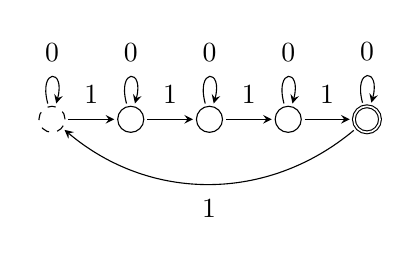
\begin{tikzpicture}
  [bend angle=40,every node/.style={draw,circle}]

  \tikzstyle{initial} = [dashed]

  \node[initial]   (1) at (1,0) {};
  \node            (2) at (2,0) {};
  \node            (3) at (3,0) {};
  \node            (4) at (4,0) {};
  \node[accepting] (5) at (5,0) {};

  \path[->, >=stealth, shorten > = 1pt, shorten < = 1pt]
        (1) edge              node[auto,draw=none] {1} (2) 
        (2) edge              node[auto,draw=none] {1} (3)
        (3) edge              node[auto,draw=none] {1} (4)
        (4) edge              node[auto,draw=none] {1} (5)
        (1) edge [loop above] node[auto,draw=none] {0} (1)
        (2) edge [loop above] node[auto,draw=none] {0} (2)
        (3) edge [loop above] node[auto,draw=none] {0} (3)
        (4) edge [loop above] node[auto,draw=none] {0} (4)
        (5) edge [loop above] node[auto,draw=none] {0} (5)
        (5) edge [bend left]  node[auto,draw=none] {1} (1);
\end{tikzpicture}
\caption{The target automaton} \label{fig:target}
\end{figure}

\begin{figure}
\centering
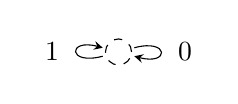
\begin{tikzpicture}
  [bend angle=40,every node/.style={draw,circle}]

  \tikzstyle{initial} = [dashed]

  \node[initial]   (1) at (1,0) {};

  \path[->, >=stealth, shorten > = 1pt, shorten < = 1pt]
        (1) edge [loop right] node[auto,draw=none] {0} (2) 
        (1) edge [loop left]  node[auto,draw=none] {1} (2);
\end{tikzpicture}
\caption{First hypothesis} \label{fig:hypoth_1}
\end{figure}


\begin{tabular}{ | l || c | }
\hline
      & $\lambda$ \\ \hline \hline
$\lambda$   & $0$ \\ \hline \hline
$0$     & $0$ \\
$1$     & $0$ \\
\hline
\end{tabular}
\quad
\begin{tabular}{ | l || c | }
\hline
      & $\lambda$ \\ \hline \hline
$\lambda$   & $0$ \\ 
$1$     & $0$ \\ 
$11$    & $0$ \\ 
$111$   & $1$ \\ \hline \hline
$0$     & $0$ \\
$10$    & $0$ \\
$110$     & $0$ \\
$1110$    & $1$ \\
$1111$    & $0$ \\
\hline
\end{tabular}
\quad
\begin{tabular}{ | l || c | c | }
\hline
      & $\lambda$   & $1$ \\ \hline \hline
$\lambda$   & $0$       & $0$ \\ 
$1$     & $0$       & $0$ \\ 
$11$    & $0$       & $1$ \\ 
$111$   & $1$       & $1$ \\ \hline \hline
$0$     & $0$       & $0$ \\
$10$    & $0$       & $0$ \\
$110$     & $0$       & $0$ \\
$1110$    & $1$       & $1$ \\
$1111$    & $0$       & $0$ \\
\hline
\end{tabular}
\quad
\begin{tabular}{ | l || c | c | c | }
\hline
      & $\lambda$   & $1$   & $11$ \\ \hline \hline
$\lambda$   & $0$       & $0$   & $0$ \\ 
$1$     & $0$       & $0$   & $1$ \\ 
$11$    & $0$       & $1$   & $0$ \\ 
$111$   & $1$       & $1$   & $0$ \\ \hline \hline
$0$     & $0$       & $0$   & $0$ \\
$10$    & $0$       & $0$   & $1$ \\
$110$     & $0$       & $0$   & $0$ \\
$1110$    & $1$       & $1$   & $0$ \\
$1111$    & $0$       & $0$   & $0$ \\
\hline
\end{tabular}

\todo{use better layout the figures and tables}




\end{document}

%%% Local Variables:
%%% mode: latex
%%% TeX-master: "main"
%%% End: